\section{Results} \label{sec:results}
% focus on the results, not on the analysis

% intro
Within this chapter, we present the crucial component of our study,
where we distill the essence of the extended PPI network by identifying the top 10 genes that stand out as significant contributors.
These genes have been selected based on their high connectivity and substantial change in gene activity within the network.


% Presentation of the 10 Genes
To identify the most significant genes, we extracted the top 10 genes with the highest PageRank scores from the list of relevant genes,
as shown in Figure~\ref{fig:03_03_df_pagerank_relevant}.
These genes are not only highly connected within the network but also exhibit a substantial change in gene activity.

\begin{figure}[h]
    \centering
    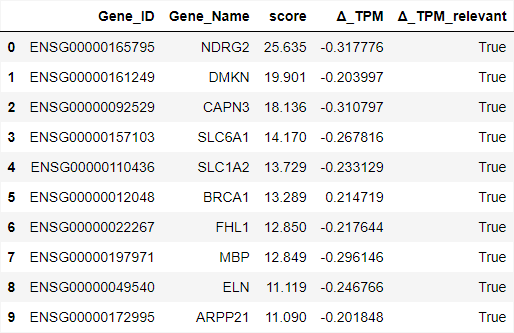
\includegraphics[height=\dfheightdouble]{figures/03_03_df_pagerank_relevant}
    \caption{Top 10 genes with the highest PageRank scores and a significant change in gene activity}
    \label{fig:03_03_df_pagerank_relevant}
\end{figure}


% Outro
The 10 genes presented here have been identified as key players in the extended PPI network related to lung cancer.
By extracting these top-scoring genes, we not only highlight potential biomarkers but also
shed light on the intricate relationships within this complex biological system.
To further validate these findings, we will conduct a detailed analysis of the current literature and compare our results with existing studies.
